\documentclass[journal,twocolumn]{IEEEtran}
%
\makeatletter
\makeatother
\usepackage{setspace}
\usepackage{gensymb}
\usepackage{xcolor}
\usepackage{caption}
%\usepackage{stackengine}
%\usepackage{subcaption}
%\doublespacing
\singlespacing



\usepackage{graphicx}
\graphicspath{ {./images}  }
%\usepackage{amssymb}
%\usepackage{relsize}
\usepackage[cmex10]{amsmath}
\usepackage{mathtools}
%\usepackage{amsthm}
\interdisplaylinepenalty=2500
%\savesymbol{iint}
%\usepackage{txfonts}
%\restoresymbol{TXF}{iint}
\usepackage{wasysym}
\usepackage{amsthm}
\usepackage{mathrsfs}
\usepackage{txfonts}
\usepackage{stfloats}
\usepackage{cite}
\usepackage{cases}
\usepackage{mathtools}
\usepackage{subfig}
\usepackage{enumerate}	
\usepackage{enumitem}
\usepackage{amsmath}
%\usepackage{xtab}
\usepackage{longtable}
\usepackage{multirow}
%\usepackage{algorithm}
%\usepackage{algpseudocode}
\usepackage{enumitem}
\usepackage{mathtools}
\usepackage[colorlinks=true, allcolors=blue]{hyperref}
%\usepackage{iithtlc}
\usepackage{tikz}
\usetikzlibrary{shapes,arrows}

%\usetikzlibrary{arrows.meta,calc,positioning}
%\usepackage[framemethod=tikz]{mdframed}
\usepackage{listings}
    \usepackage[latin1]{inputenc}                                 %%
    \usepackage{color}                                            %%
    \usepackage{array}                                            %%
    \usepackage{longtable}                                        %%
    \usepackage{calc}                                             %%
    \usepackage{multirow}                                         %%
    \usepackage{hhline}                                           %%
    \usepackage{ifthen}                                           %%
  %optionally (for landscape tables embedded in another document): %%
    \usepackage{lscape}     


%\usepackage{stmaryrd}


%\usepackage{wasysym}
%\newcounter{MYtempeqncnt}
\DeclareMathOperator*{\Res}{Res}
%\renewcommand{\baselinestretch}{4}
%\setcounter{secnumdepth}{4}
\renewcommand\thesection{\arabic{section}}
\renewcommand\thesubsection{\thesection.\arabic{subsection}}
\renewcommand\thesubsubsection{\thesubsection.\arabic{subsubsection}}
%\renewcommand\thesubsubsubsection{\thesubsubsection.\arabic{subsubsubsection}}

%\renewcommand\thesectiondis{\arabic{section}}
%\renewcommand\thesubsectiondis{\thesectiondis.\arabic{subsection}}
%\renewcommand\thesubsubsectiondis{\thesubsectiondis.\arabic{subsubsection}}
%\renewcommand\thesubsubsubsectiondis{\thesubsubsectiondis.\arabic{subsubsubsection}}
% correct bad hyphenation here
\hyphenation{Future Wireless communications}

%\lstset{
%language=C,
%frame=single, 
%breaklines=true
%}

%\lstset{
	%%basicstyle=\small\ttfamily\bfseries,
	%%numberstyle=\small\ttfamily,
	%language=Octave,
	%backgroundcolor=\color{white},
	%%frame=single,
	%%keywordstyle=\bfseries,
	%%breaklines=true,
	%%showstringspaces=false,
	%%xleftmargin=-10mm,
	%%aboveskip=-1mm,
	%%belowskip=0mm
%}

%\surroundwithmdframed[width=\columnwidth]{lstlisting}
\def\inputGnumericTable{}                                 %%

\lstset{
%language=python,
frame=single, 
breaklines=true,
columns=fullflexible
}

 

\begin{document}
%
\tikzstyle{block} = [rectangle, draw,
text width=7em, text centered, minimum height=4em]
\tikzstyle{sum} = [draw, circle, node distance=3cm]
\tikzstyle{input} = [coordinate]
\tikzstyle{output} = [coordinate]
\tikzstyle{pinstyle} = [pin edge={to-,thin,black}]
\tikzstyle{line} = [draw, -latex']
\theoremstyle{definition}
\newtheorem{theorem}{Theorem}[section]
\newtheorem{problem}{Problem}
\newtheorem{proposition}{Proposition}[section]
\newtheorem{lemma}{Lemma}[section]
\newtheorem{corollary}[theorem]{Corollary}
\newtheorem{example}{Example}[section]
\newtheorem{definition}{Definition}[section]
%\newtheorem{algorithm}{Algorithm}[section]
%\newtheorem{cor}{Corollary}
\newcommand{\BEQA}{\begin{eqnarray}}
\newcommand{\EEQA}{\end{eqnarray}}
\newcommand{\define}{\stackrel{\triangle}{=}}
\bibliographystyle{IEEEtran}
%\bibliographystyle{ieeetr}
\providecommand{\nCr}[2]{\,^{#1}C_{#2}} % nCr
\providecommand{\nPr}[2]{\,^{#1}P_{#2}} % nPr
\providecommand{\mbf}{\mathbf}
\providecommand{\pr}[1]{\ensuremath{\Pr\left(#1\right)}}
\providecommand{\qfunc}[1]{\ensuremath{Q\left(#1\right)}}
\providecommand{\sbrak}[1]{\ensuremath{{}\left[#1\right]}}
\providecommand{\lsbrak}[1]{\ensuremath{{}\left[#1\right.}}
\providecommand{\rsbrak}[1]{\ensuremath{{}\left.#1\right]}}
\providecommand{\brak}[1]{\ensuremath{\left(#1\right)}}
\providecommand{\lbrak}[1]{\ensuremath{\left(#1\right.}}
\providecommand{\rbrak}[1]{\ensuremath{\left.#1\right)}}
\providecommand{\cbrak}[1]{\ensuremath{\left\{#1\right\}}}
\providecommand{\lcbrak}[1]{\ensuremath{\left\{#1\right.}}
\providecommand{\rcbrak}[1]{\ensuremath{\left.#1\right\}}}
\theoremstyle{remark}
\newtheorem{rem}{Remark}
\newcommand{\sgn}{\mathop{\mathrm{sgn}}}
\providecommand{\abs}[1]{\left\vert#1\right\vert}
\providecommand{\res}[1]{\Res\displaylimits_{#1}} 
\providecommand{\norm}[1]{\lVert#1\rVert}
\providecommand{\mtx}[1]{\mathbf{#1}}
\providecommand{\mean}[1]{E\left[ #1 \right]}
\providecommand{\fourier}{\overset{\mathcal{F}}{ \rightleftharpoons}}
%\providecommand{\hilbert}{\overset{\mathcal{H}}{ \rightleftharpoons}}
\providecommand{\system}{\overset{\mathcal{H}}{ \longleftrightarrow}}
	%\newcommand{\solution}[2]{\textbf{Solution:}{#1}}
\newcommand{\solution}{\noindent \textbf{Solution: }}
\newcommand{\myvec}[1]{\ensuremath{\begin{pmatrix}#1\end{pmatrix}}}
\providecommand{\dec}[2]{\ensuremath{\overset{#1}{\underset{#2}{\gtrless}}}}
\DeclarePairedDelimiter{\ceil}{\lceil}{\rceil}
%\numberwithin{equation}{subsection}
\numberwithin{equation}{section}
%\numberwithin{problem}{subsection}
%\numberwithin{definition}{subsection}
%\makeatletter
%\@addtoreset{figure}{section}
%\makeatother
\let\StandardTheFigure\thefigure
%\renewcommand{\thefigure}{\theproblem.\arabic{figure}}
%\renewcommand{\thefigure}{\thesection}
%\numberwithin{figure}{subsection}
%\numberwithin{equation}{subsection}
%\numberwithin{equation}{section}
%\numberwithin{equation}{problem}
%\numberwithin{problem}{subsection}
%\numberwithin{problem}{section}
%%\numberwithin{definition}{subsection}
%\makeatletter
%\@addtoreset{figure}{problem}
%\makeatother
%\makeatletter
%\@addtoreset{table}{problem}
%\makeatother
\let\StandardTheFigure\thefigure
\let\StandardTheTable\thetable
\let\vec\mathbf
%%\renewcommand{\thefigure}{\theproblem.\arabic{figure}}
%\renewcommand{\thefigure}{\theproblem}
%%\numberwithin{figure}{section}
%%\numberwithin{figure}{subsection}
\def\putbox#1#2#3{\makebox[0in][l]{\makebox[#1][l]{}\raisebox{\baselineskip}[0in][0in]{\raisebox{#2}[0in][0in]{#3}}}}
     \def\rightbox#1{\makebox[0in][r]{#1}}
     \def\centbox#1{\makebox[0in]{#1}}
     \def\topbox#1{\raisebox{-\baselineskip}[0in][0in]{#1}}
     \def\midbox#1{\raisebox{-0.5\baselineskip}[0in][0in]{#1}}
\title{ 
%	\logo{
5G NR LDPC Encoder and Decoder 
%	}
}
\author{YADATI KRISHNA}% <-this % stops a space
% make the title area
\maketitle
\tableofcontents
\section{\textbf{Introduction}}
5G NR (New Radio) is the latest wireless communication standard that supports higher data rates, lower latency, and increased reliability. LDPC (Low-Density Parity-Check) is a forward error correction (FEC) technique used in 5G NR to improve the reliability of data transmission.\\

5G NR (New Radio) uses Low-Density Parity-Check (LDPC) codes for forward error correction (FEC) to improve the reliability of data transmission over wireless channels. LDPC codes are linear block codes that have a sparse parity-check matrix. The parity-check matrix is designed to have a low density of 1's, which means that only a small fraction of the bits in the matrix are 1's.\\

The 5G NR LDPC codes are designed to have a high coding gain and low error rates while maintaining low latency and complexity. The coding gain is the ratio of the signal-to-noise ratio (SNR) required for a non-coded system to achieve a certain bit error rate (BER) compared to the SNR required for a coded system to achieve the same BER. The higher the coding gain, the more robust the code is against channel noise and interference.\\

The 5G NR LDPC codes are specified by the 3GPP (Third Generation Partnership Project) and include several code rates ranging from 1/5 to 5/6. The code rates determine the amount of redundancy added to the original data to create the codeword. Higher code rates add more redundancy, which results in a more robust code but also increases the latency of the transmission.\\

The 5G NR LDPC codes have a block size of 8448 bits and are designed to be flexible and adaptable to different channel conditions. The code rate and the number of iterations used in the decoding process can be adjusted based on the channel conditions to optimize the trade-off between coding gain, latency, and complexity.\\

Overall, the 5G NR LDPC codes are a crucial component of the 5G NR communication system, and their performance has a significant impact on the reliability and efficiency of data transmission over wireless channels.
\section{\textbf{5G NR LDPC Encoder}}
The 5G NR (New Radio) encoder is responsible for encoding information bits into a larger codeword to improve the reliability of data transmission. The 5G NR standard uses a specific type of forward error correction (FEC) technique called LDPC (Low-Density Parity-Check) for error correction. The 5G NR LDPC encoder adds redundant bits to the original information bits to create the codeword.\\

The 5G NR LDPC encoder uses a parity-check matrix to determine the redundant bits to add to the information bits. The matrix is designed to have a low-density of 1's, which means that only a small fraction of the bits in the matrix are 1's. This reduces the complexity of the encoder and decoder while still providing high coding gain and low error rates.\\

The 5G NR LDPC encoder can operate at different code rates, which determines the amount of redundancy added to the information bits. The higher the code rate, the more redundancy is added, which results in a more robust codeword but also increases the latency of the transmission.\\

The 5G NR encoder also includes other features such as rate matching and code block segmentation. Rate matching is used to adjust the size of the codeword to match the modulation and channel coding scheme used for transmission. Code block segmentation is used to divide the information bits into smaller code blocks, which can be processed and encoded separately.\\

Overall, the 5G NR encoder is a critical component of the communication system, and its performance impacts the reliability and efficiency of data transmission over 5G networks.

\subsection{\textbf{
5G-NR LDPC Channel coding}}
Based on my interpretation from {\href{https://www.etsi.org/deliver/etsi_ts/138200_138299/138212/17.01.00_60/ts_138212v170100p.pdf}{3GPP Specification 38.212} Rel 15 (Multiplexing and channel coding), I had put together the procedure on how LDPC Base Graph selection and coding happens.
\begin{enumerate}
  \item For transmission of a DL transport block , a transport block CRC is first appended to provide error detection, followed by a LDPC base graph selection.
  \item   NR supports two LDPC base graphs, one for small transport blocks and one for larger transport blocks.
   \item  Then transport block is segmented into code blocks and code block CRC attachment is performed.
   \item  Each code block is individually LDPC encoded. The LDPC coded blocks are then individually rate matched.
  \item   Finally, code block concatenation is performed to create a codeword for transmission. Up to 2 code words can be transmitted simultaneously. 
    \end{enumerate}
 \subsection{\textbf{
LDPC Base Graphs}}   
    There are two types of Base Graphs standardized in the specification, {\href{https://www.etsi.org/deliver/etsi_ts/138200_138299/138212/17.01.00_60/ts_138212v170100p.pdf}{3GPP Specification 38.212} (Multiplexing and channel coding).Base Graph is a Matrix where each of the entries can be further expanded based on the expansion factor Zc.
\begin{enumerate}
  \item  Base Graph 1 (BG1) : With Matrix size 46X68 entries For Large Transport Block 
  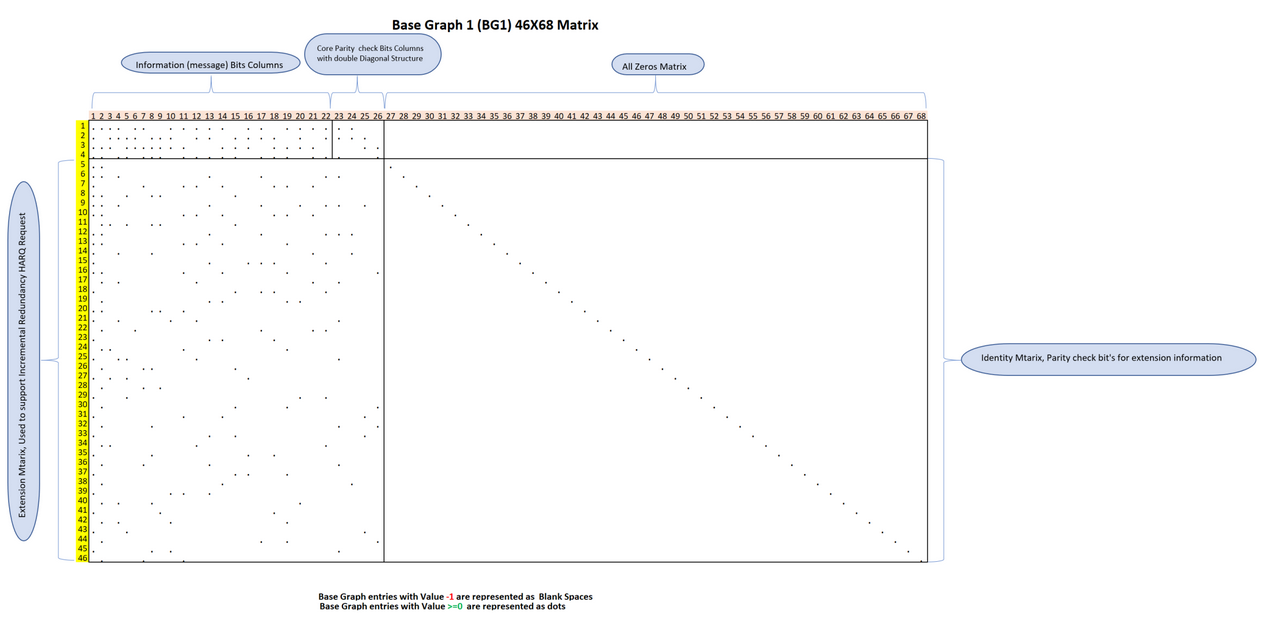
\includegraphics[width=\columnwidth]{../figs/bg1.png} 

  \item  Base Graph 2 (BG2): With matrix size 42X52 entries For Smaller Transport Block
  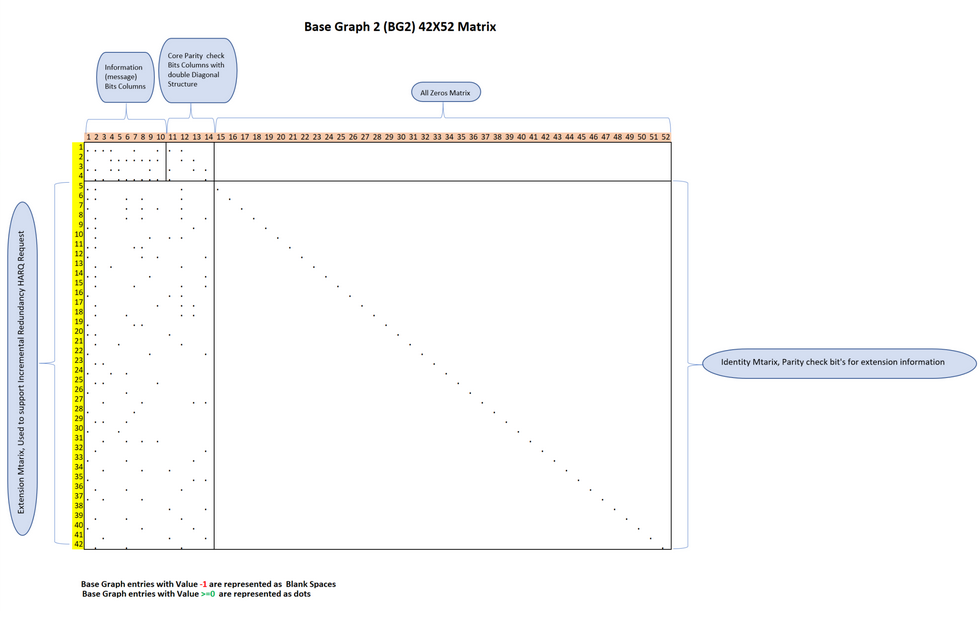
\includegraphics[width=\columnwidth]{../figs/bg2.png} 
      \end{enumerate}
\end{document}